%! Author = taj
%! Date = 7/22/25

% Preamble
\documentclass[11pt]{article}

% Packages
\usepackage{amsmath}
\usepackage{graphicx}
\usepackage{float}

\title{1. Merjenje moči mšic rok in nog}
\author{Taj Šobot}


% Document
\begin{document}
    \maketitle
    \flushleft

    V tem eksperimentu smo s pomočjo digitalnega silomera in ultrazvočnega merilnika merili moč mišic v nogah in rokah.


    \section{Meritve}
    Merive smo izvajali z orodjem "Logger Pro", merilno ploščo, s katerim smo merili silo in ultrazvočnim merilnikom, s katerim smo merili višino skokov.
    Merili smo, kako se sila spreminja s časom pri odskoku in odrivu od stene.
    Ker so meritve digitalne jih v tem poglavju nemoremo prikazati.

    \section{rezultati in grafi}
    a) Sile skakalca pri navpičnem skoku:
    \\

    Pri tem delu vaje smo skakali iz silomera in preučevali različne faze odskoka in pristanka.
    Spodaj je prikazan garf sile v odvisnosti od časa pri doskoku od merilne plošče.
    Pri pristanku nismo pristajali nazaj na merilno ploščo, da je ne bi poškodovali.
    \begin{figure}[H]
        \centering
        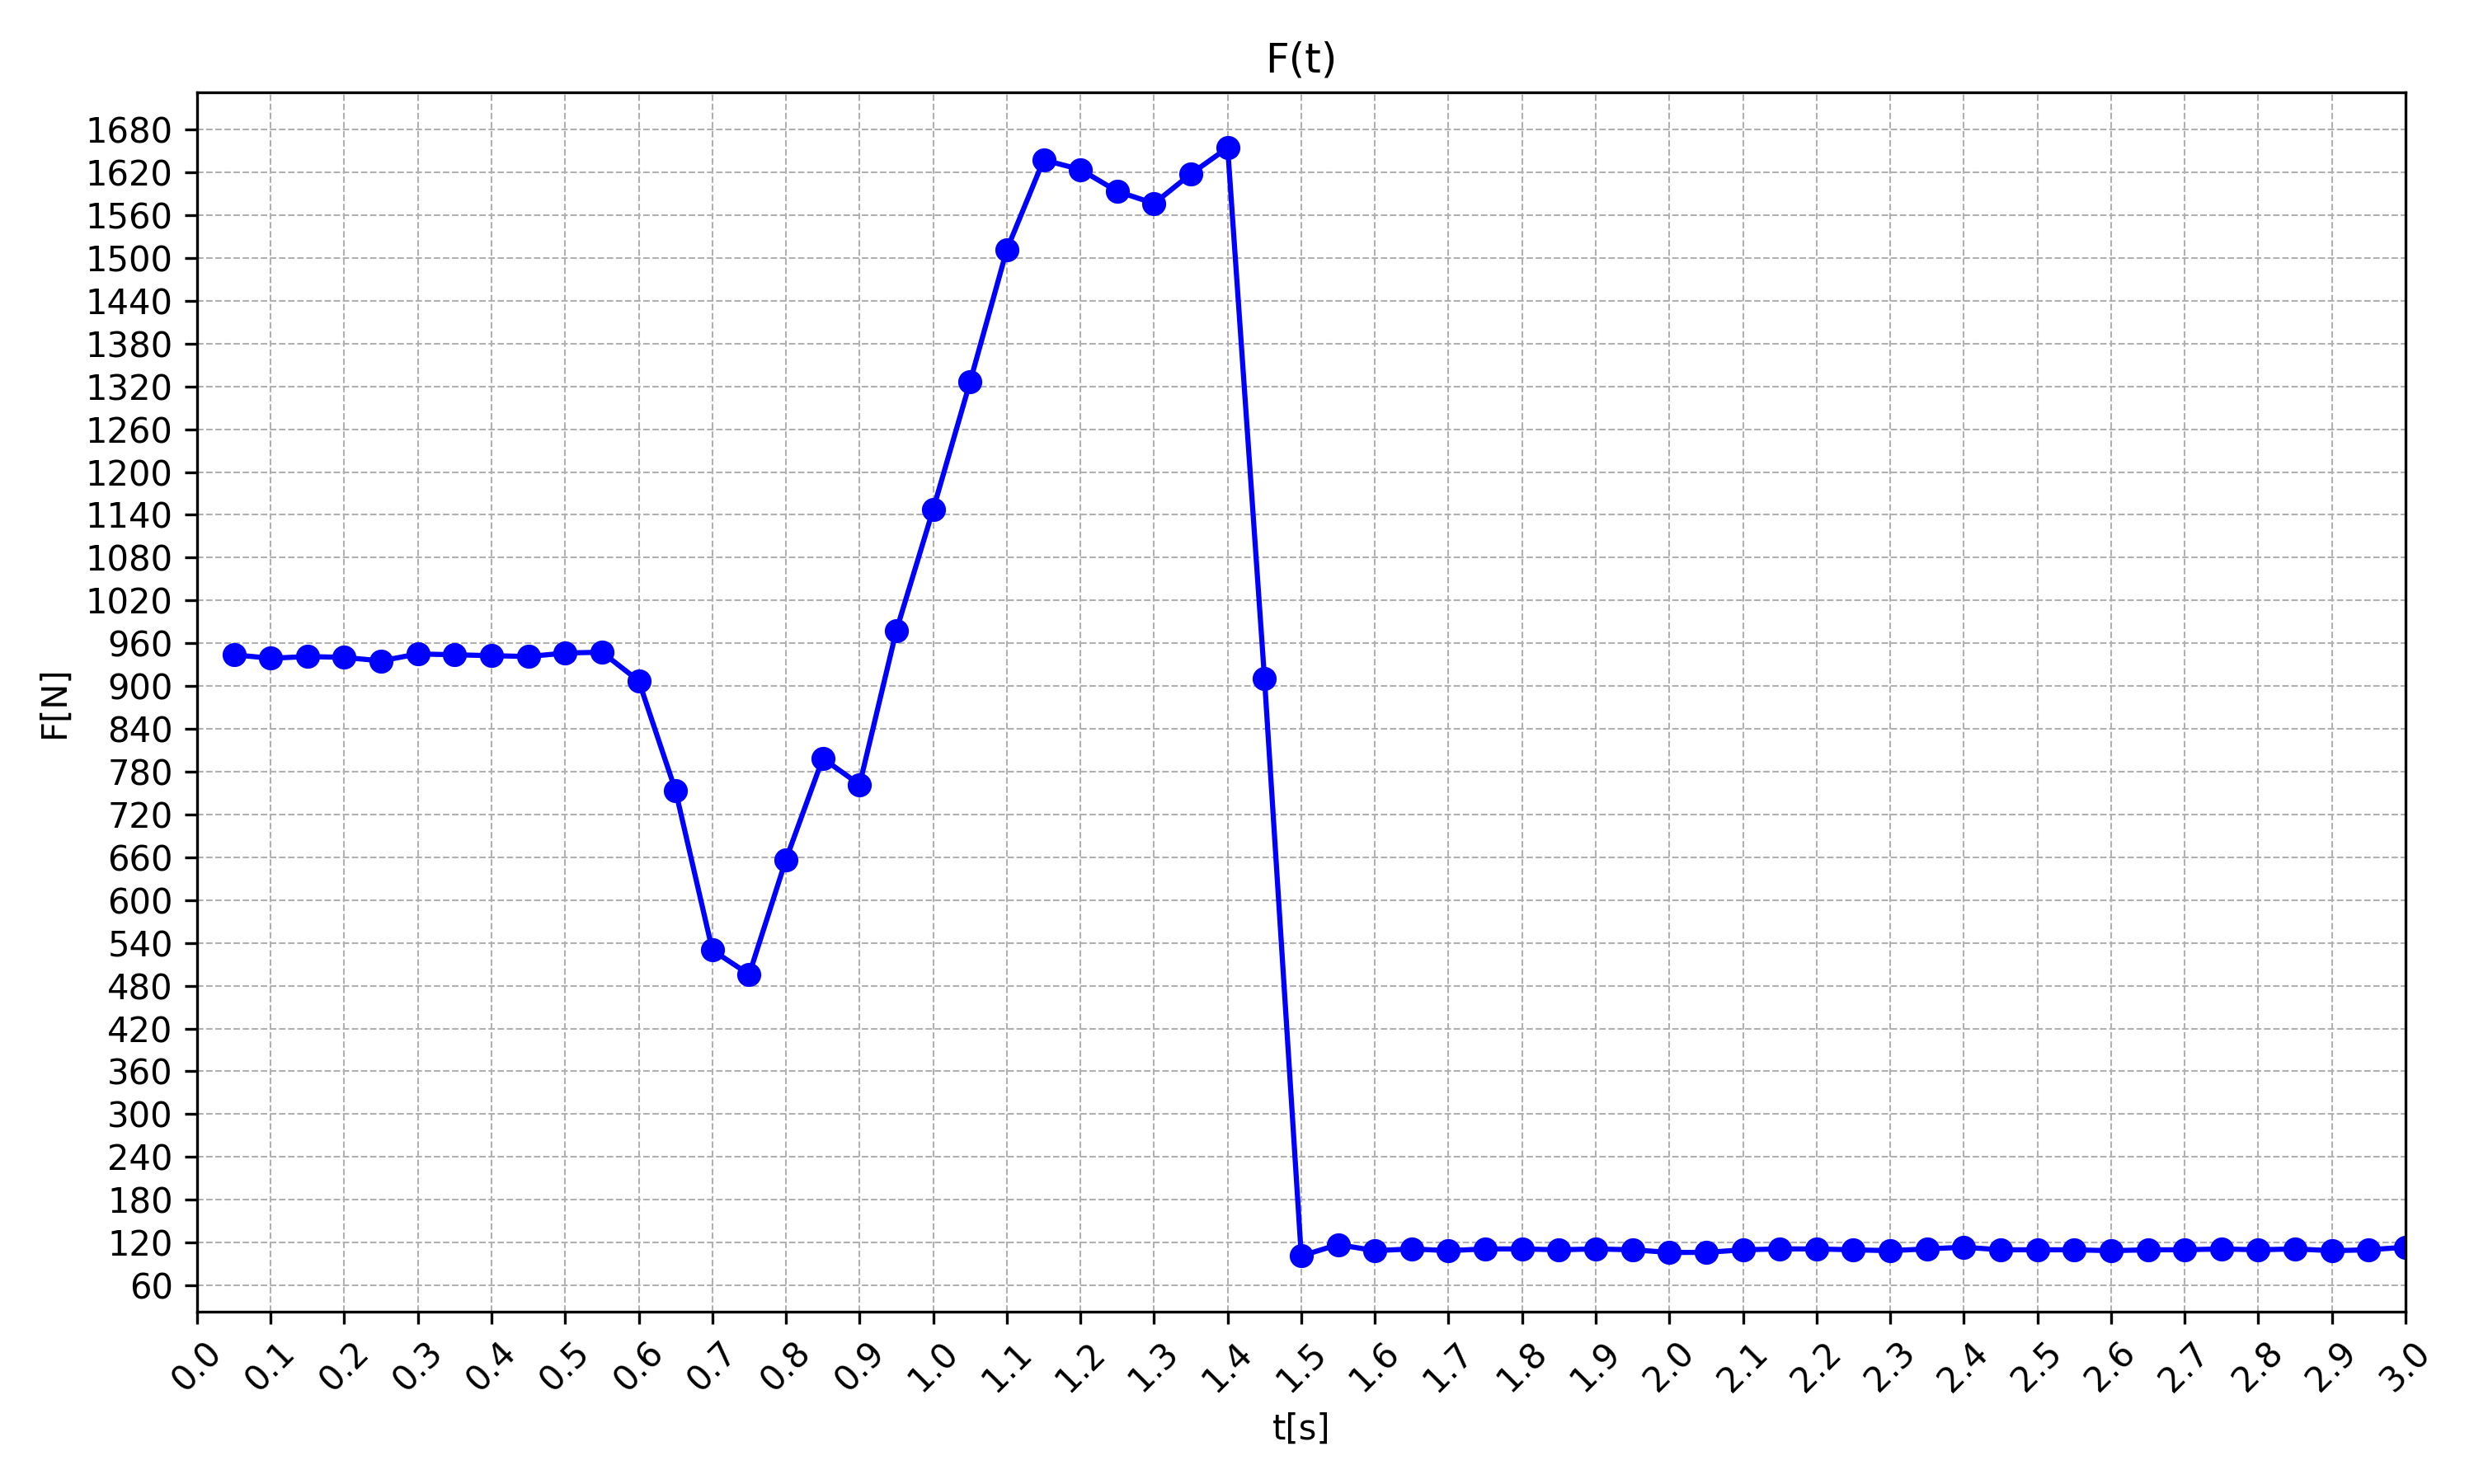
\includegraphics[width=0.9\textwidth]{TMT}
        \caption{F(t) - Taj}
        \label{fig:1}
    \end{figure}

    b)Moč in delo mišic nog skakalca pri navpičnem skoku:
    \\
    Pri tem delu vaje smo preučevali višno istega skoka z ultrazvočnim merilnikom.
    Spodaj je prikazan graf višine v odvisnosti od časa.
    \begin{figure}[H]
        \centering
        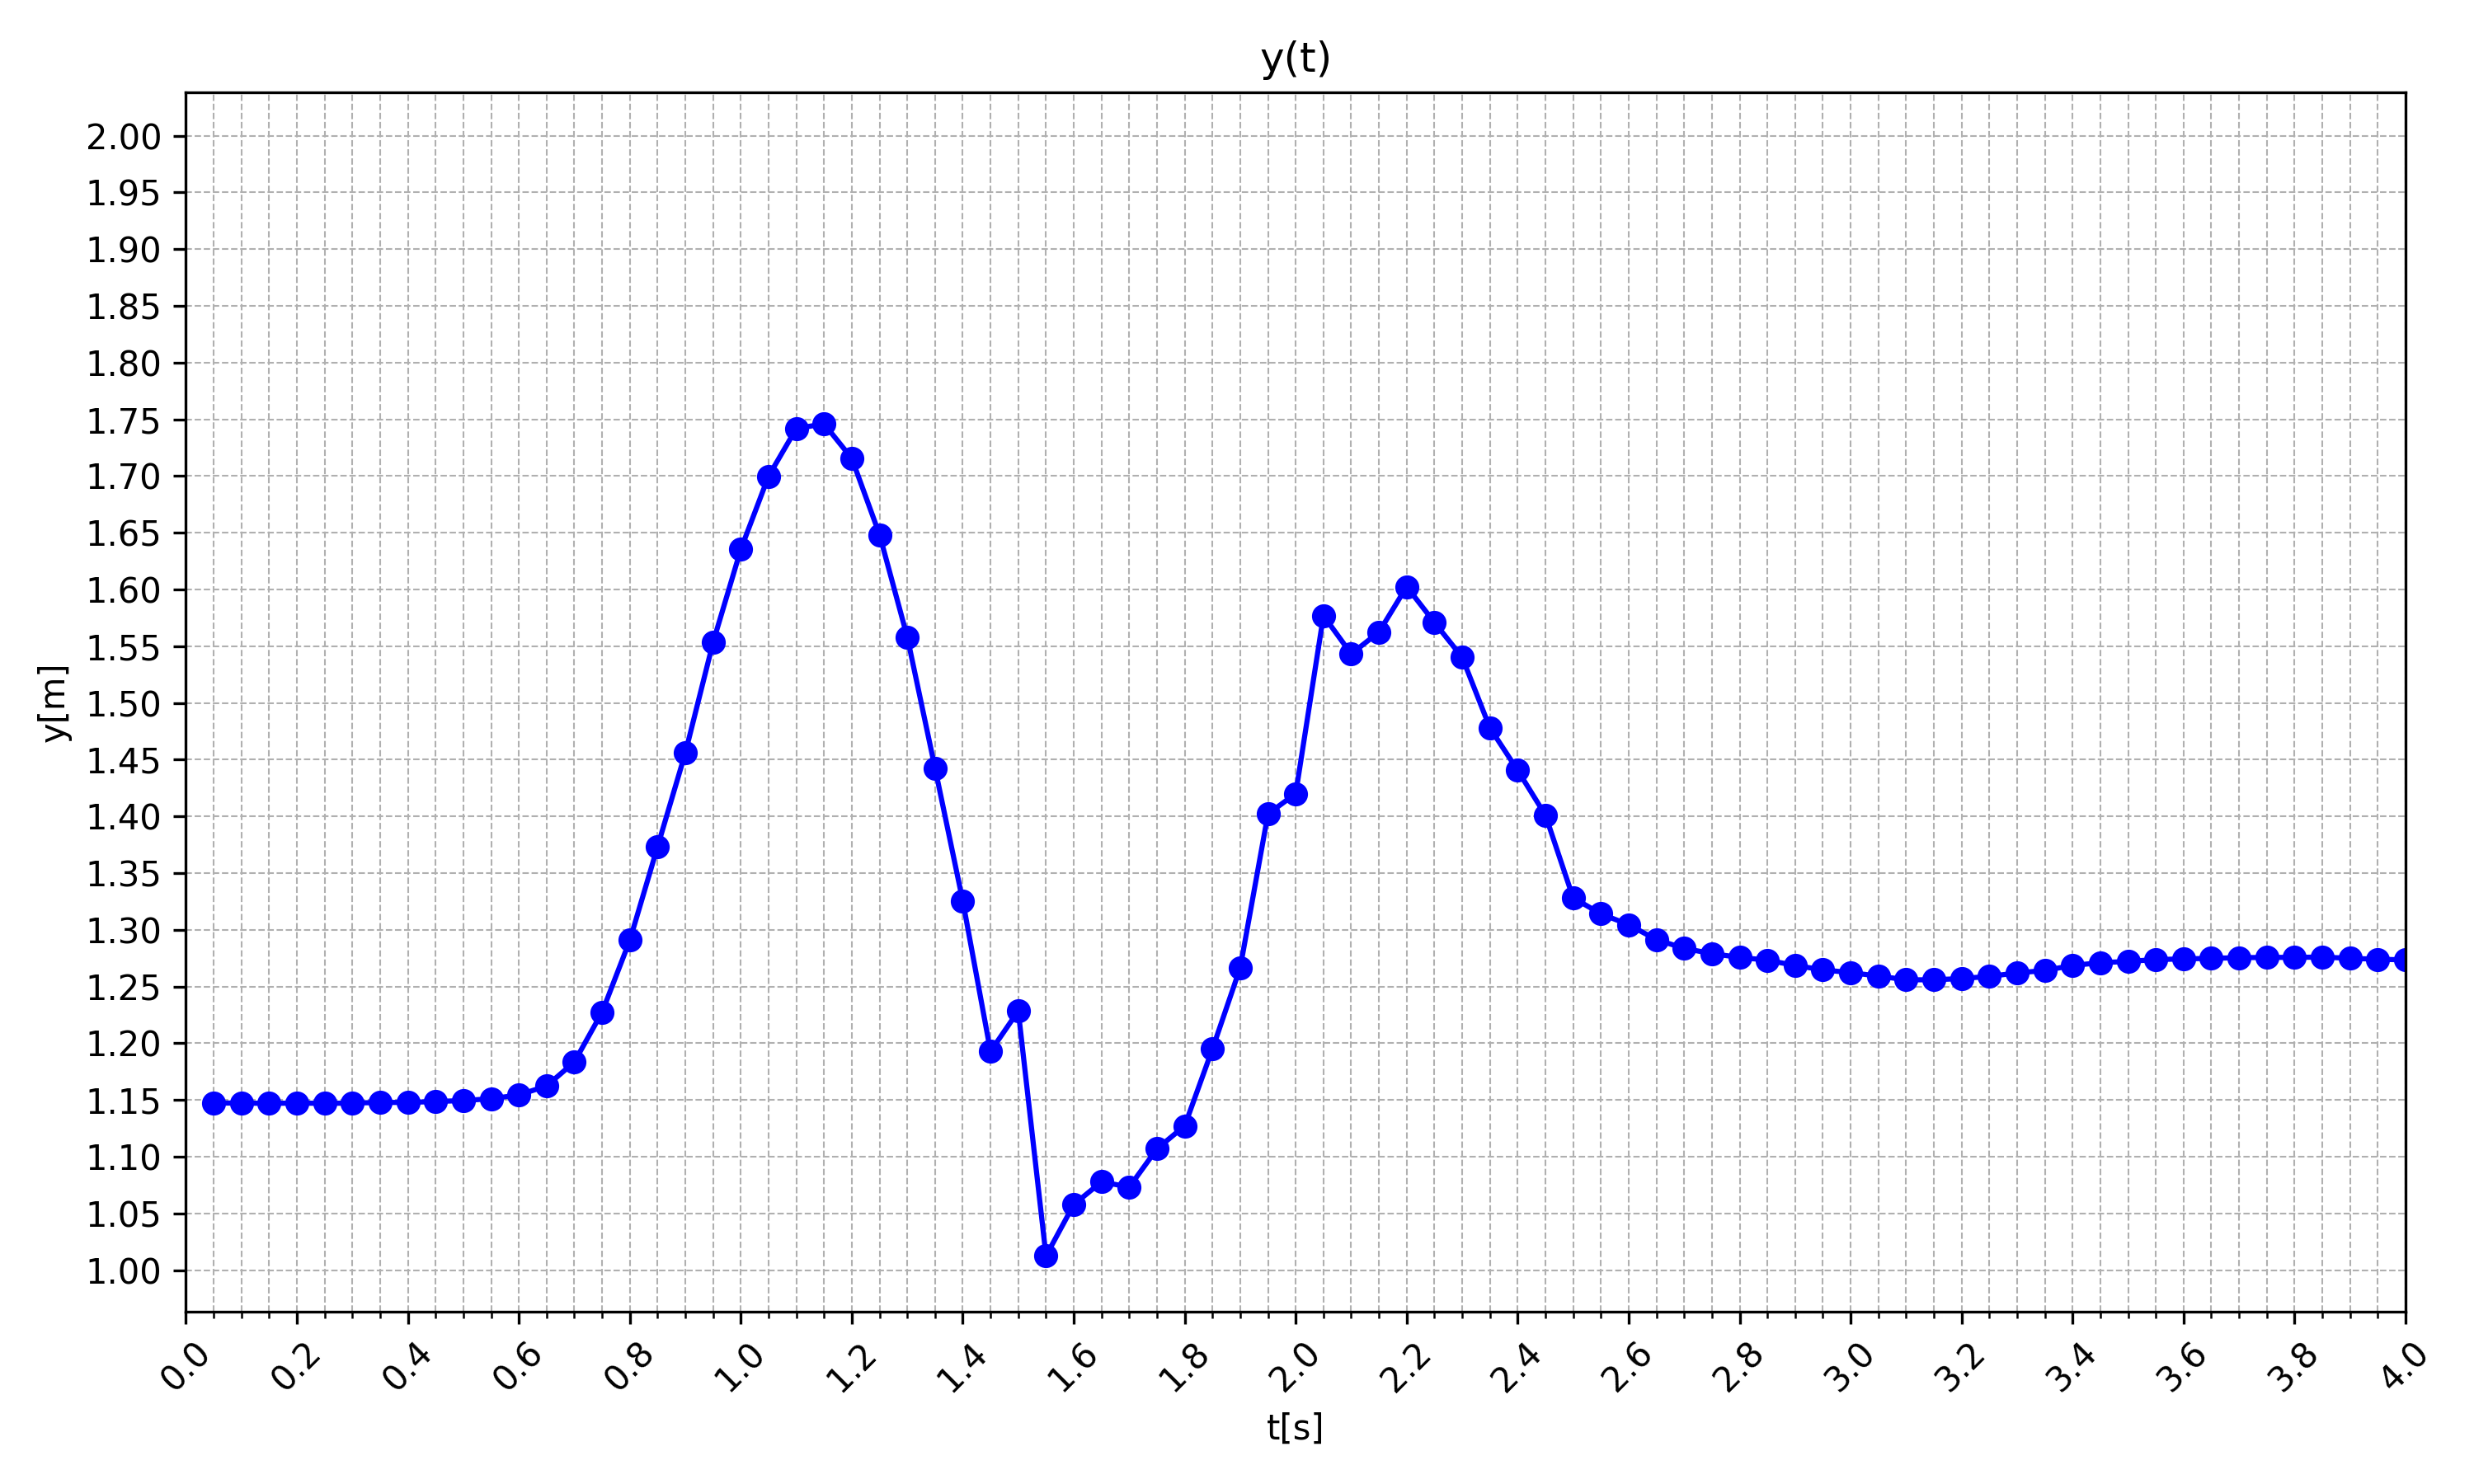
\includegraphics[width=0.9\textwidth]{TMTb}
        \caption{y(t) - Taj}
        \label{fig:2}
    \end{figure}
    iz grafa lahko odčitamo višinsko razliko H, ki je razdalja od počepa do najvišje točke skoka.
    $H = (0,75 \pm 0,01) \text{m}$.
    Z uporabo enačbe:
    \[
        A_m = mgH
    \]
    lahko izračunamo delo, ki so ga mišice opravile za skok.
    Ko vstavimo maso skakalca $m = (84,7 \pm 0,5) kg$ in gravitacijski pospešek $g = (9,81 \pm 0,01) \frac{m}{s^2}$:
    \[
        A_m = (623 \pm 3) J
    \]
    Iz grafa tudi odčitamo čas odriva $t_o = (0.45 \pm 0.05) s$.
    Tako dobimo moč mišic iz enačbe:
    \[
        W_m = \frac{A_m}{t_o} = (1600 \pm 200) W
    \]

    c) Merjenje moči mišic rok:
    \\
    Pri tem delu vaj smo se odrivali od deske in merili silo, ki je na to delovala.
    Tako bomo lahko izračunali še moč rok.

    Spodaj je graf naše meritve (sile v odvisnosti od časa):

    \begin{figure}[H]
        \centering
        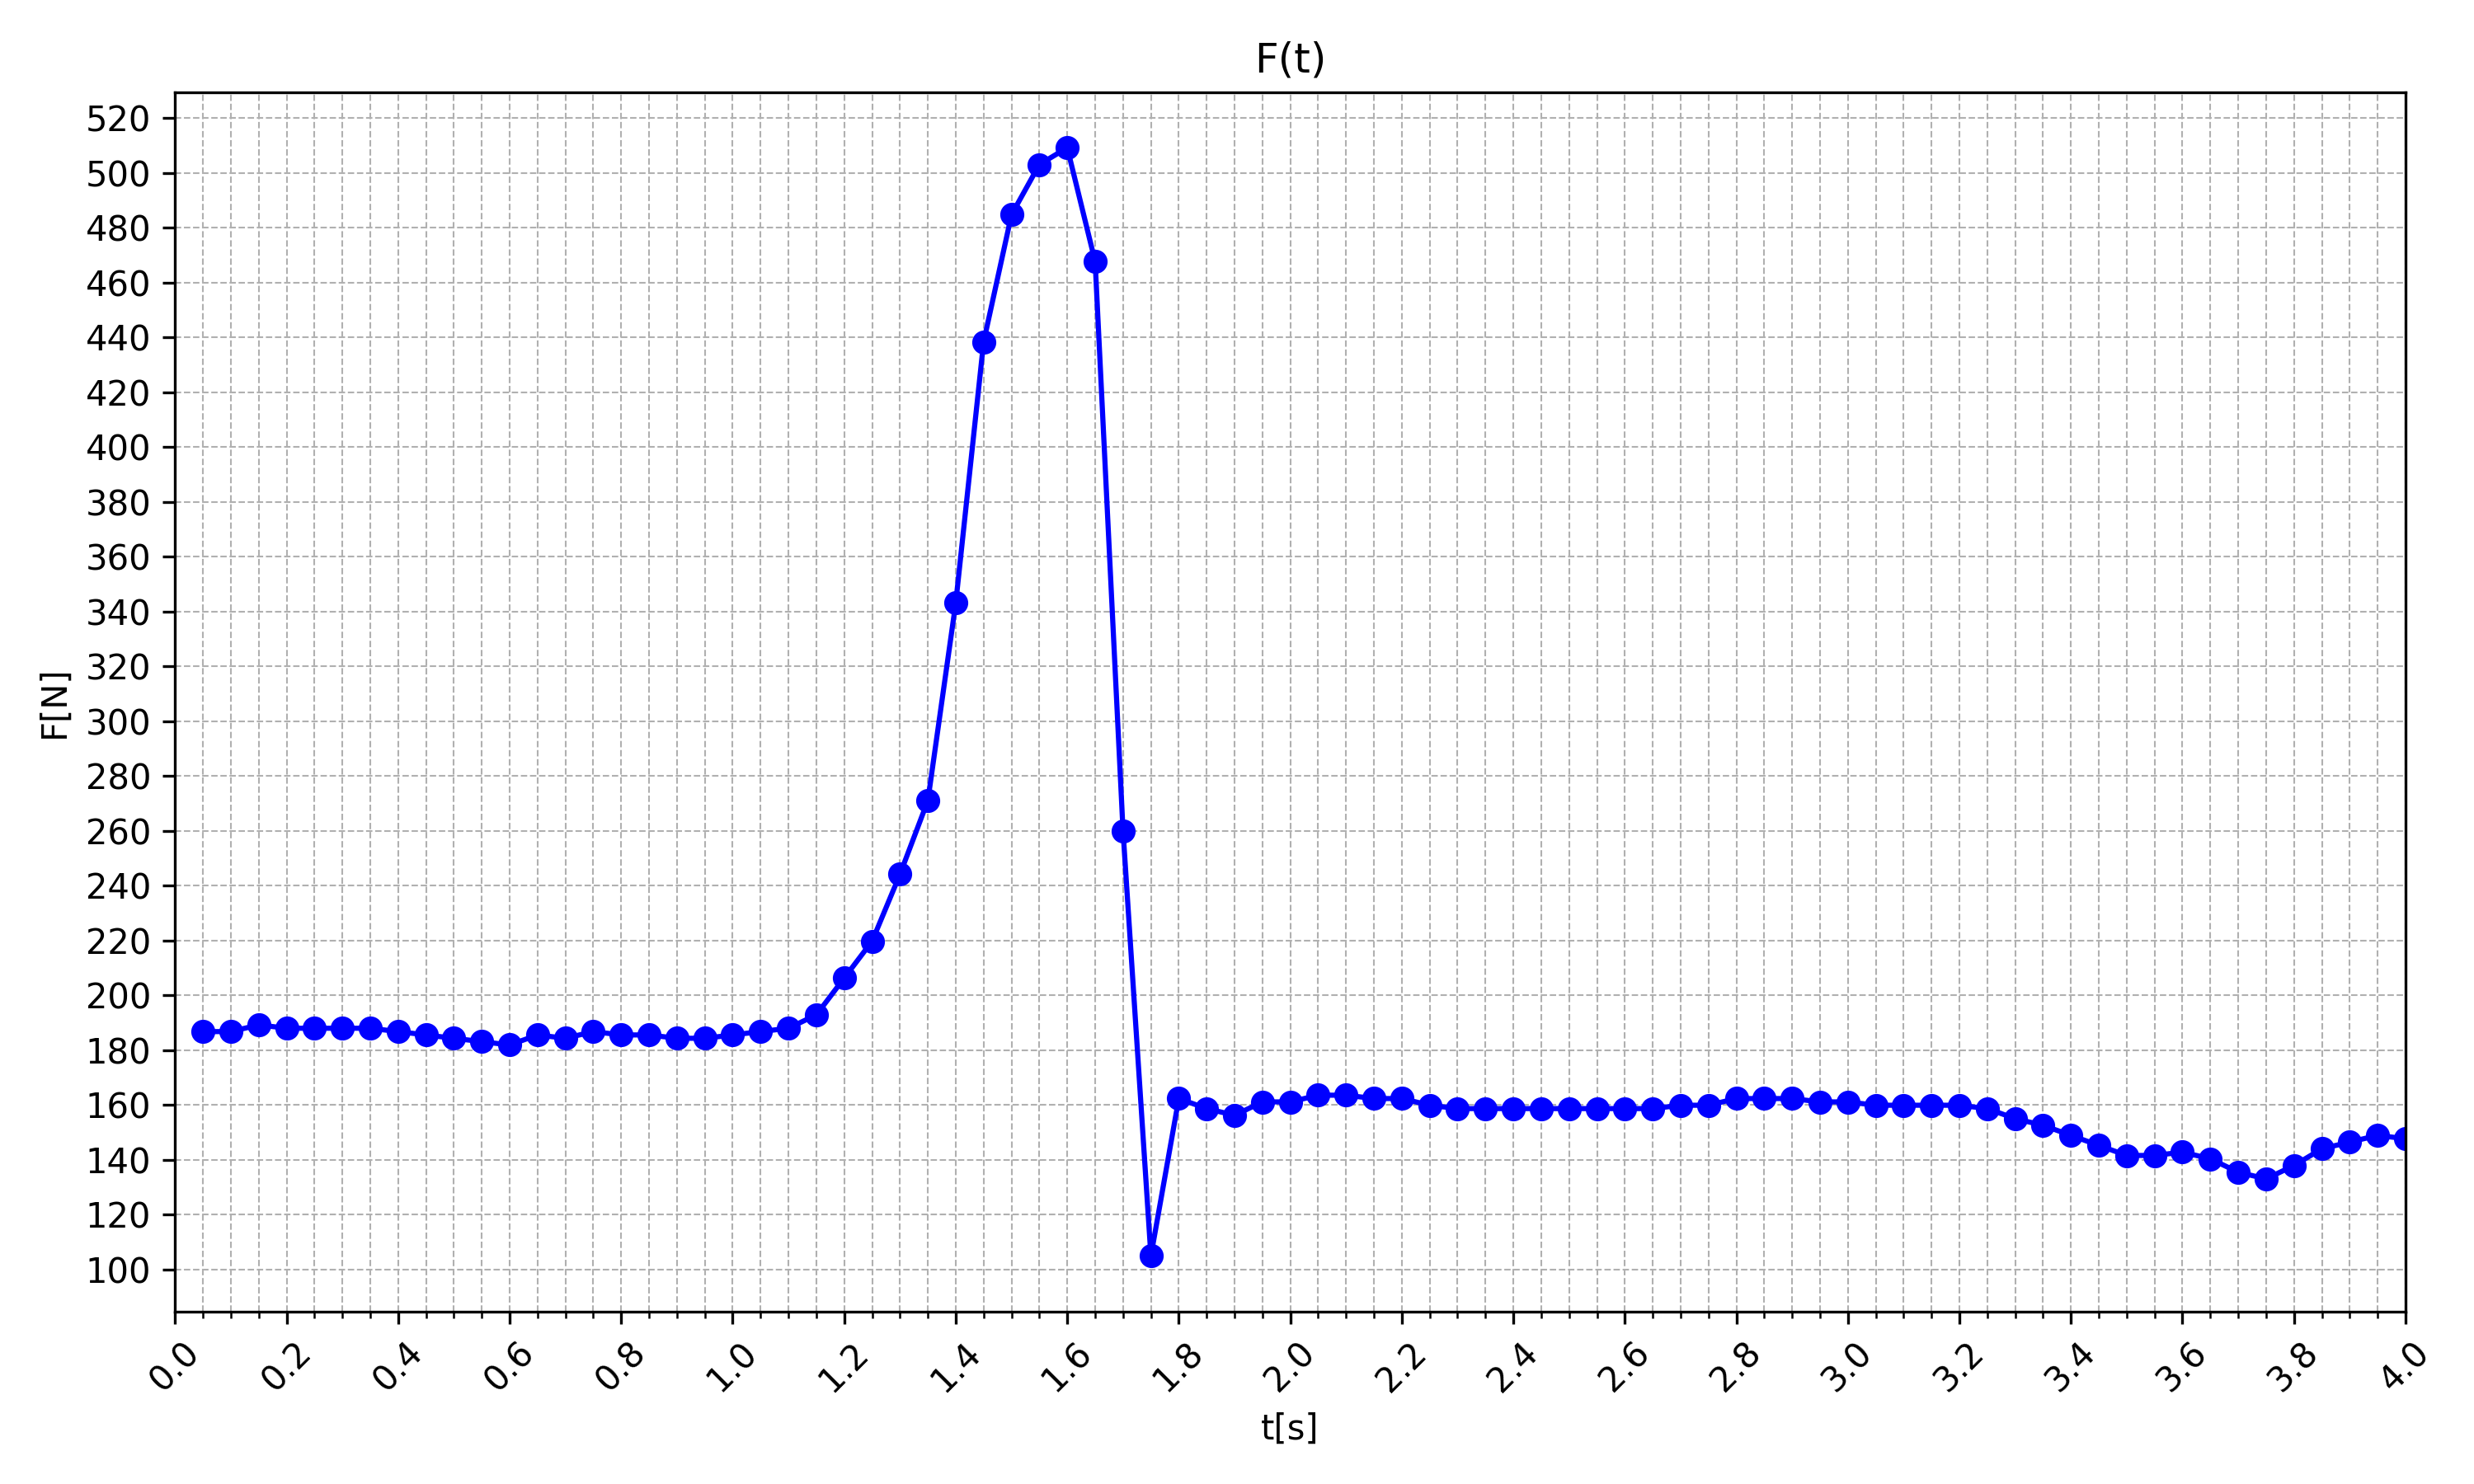
\includegraphics[width=0.9\textwidth]{TMTc}
        \caption{F(t) - Taj}
        \label{fig:3}
    \end{figure}

    Tukaj nas zanima časovni interval od  14.5s do 16.5.
    Takrat se je izvajal odriv od deske.
    Sprememba gibalne količine je:
    \[
        \int_{t_1}^{t_2} F(t)\, dt = m v_k
    \]
    Ta integral lahko kvalitativno ocenimo iz grafa.
    Po tej enačbi:
    \[
        F \Delta t = m v_k
    \]
    Iz grafa ocenimo $\Delta t = (2.0 \pm 0.5 ) s$ in $F = (430 - 160 \pm 20) N$.
    (opomba: ko merilnik sile ne obremenjujemo kaže 160 N, to pomeni da moramo to odštei od odmerka)
    Masa osebe je $m = (84,7 \pm 0,5) kg$

    V spodnjo enačbo vstavimo  dobimo končno hitrost:
    \[
        v_k = \frac{F  \Delta t }{m} = (6 \pm 1) m/s
    \]
    Delo mišic je torej:
    \[
        A_m = 1/2 m v_k^2 = (1500 \mp 300) J
    \]
    In moč:
    \[
        P = \frac{A}{\Delta t} = (800 \pm 200) W
    \]


    \section{odgovori na vprašanja}
    \textit
    {1. Razmislite in razložite, zakaj ima izmerjeni časovni potek razdalje na sliki 3 maksimum ob
    času, ko je skakalec v najnižji točki počepa, in minimum v trenutku, ko se skakalec nahaja v
    najvišji točki skoka.}
    \\ Merilnik meri razdaljo od njega do skakalčeve glave.
    Ko je skakalec daleč od merilnika (v počepu) ta izmeri največjo razdaljo in obratno ko je skakalec blizu merilnika.

    \textit {2. Iz izmerjenega časovnega poteka razdalje med temenom skakalčeve glave in merilnikom
    določite delo mišic nog po enačbi (2) in moč mišic nog po enačbi (3).}
    \\
    odgovor

    \textit {3. Iz iste meritve kot pri 2. vprašanju določite tudi: hitrost ob vzletu (vzletno hitrost) in
    povprečen pospešek težišča skakalca med odrivom.}
    \\
    odgovor

    \textit {4. Izračunajte, s kolikšno povprečno silo deluje podlaga na skakalčeva stopala med odrivom.}
    \\
    odgovor

    \textit {5. Izračunajte razmerje med močjo mišic nog in močjo mišic rok}
    \\
    odgovor


\end{document}